\section{Resultat}

\subsection{Experimentkörning}
I figurerna \ref{fig:A},\ref{fig:B},\ref{fig:C} syns datan för de första fem sekundrarna av mätningar. Där är båda pendlarna med, som $\theta$ och $\phi$, samt egenmoderna $q_1,q_2$.

\begin{figure}[htbp]
    \centering
    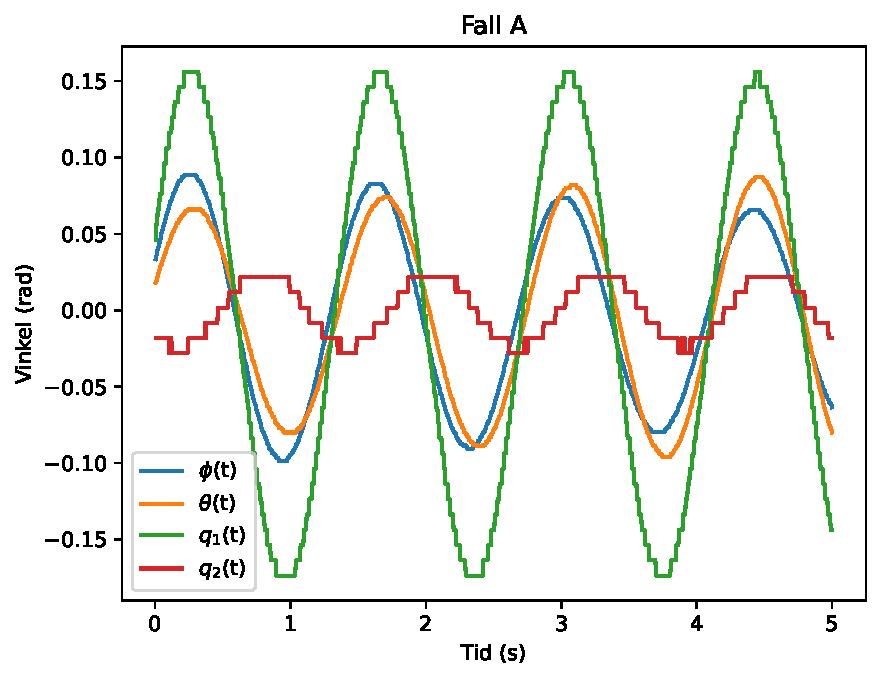
\includegraphics[width=0.7\textwidth]{plot_A.pdf}
    \caption{Mätdata från fall A.}
    \label{fig:A}
\end{figure}

\begin{figure}[htbp]
    \centering
    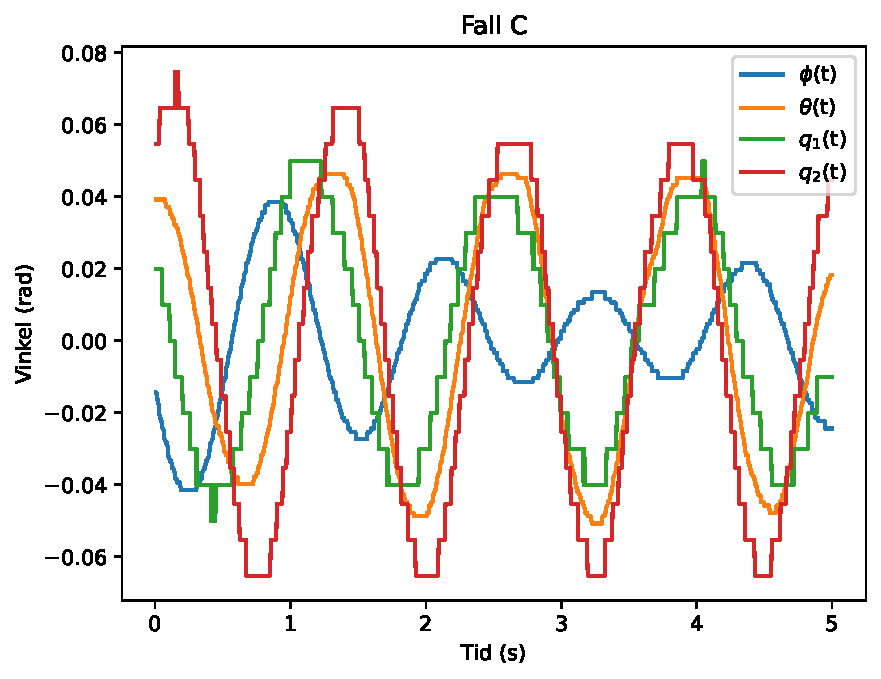
\includegraphics[width=0.7\textwidth]{plot_C.pdf}
    \caption{Mätdata från fall C.}
    \label{fig:B}
\end{figure}

\begin{figure}[htbp]
    \centering
    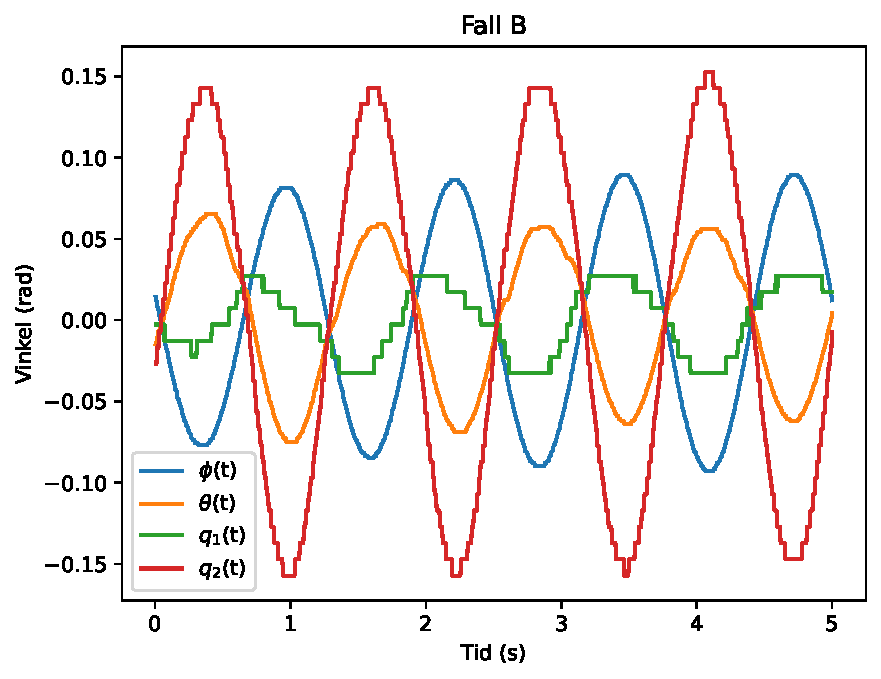
\includegraphics[width=0.7\textwidth]{plot_B.pdf}
    \caption{Mätdata från fall C.}
    \label{fig:C}
\end{figure}

Från en sinusanpassning i \emph{Capstone} fick man ut egenfrekvenserna för vardera fall:
\begin{align}
    \begin{cases}
        \omega_{A1} &= 4.52\unit{rad/s}\\
        \omega_{B1} &= 4.52\unit{rad/s}\\
        \omega_{C1} &= 4.53\unit{rad/s}
    \end{cases},\quad 
    \begin{cases}
        \omega_{A2} &= 5.05\unit{rad/s}\\
        \omega_{A2} &= 5.06\unit{rad/s}\\
        \omega_{A2} &= 5.06\unit{rad/s}
    \end{cases} \label{eq: omega cap}
\end{align}

\subsection{Mätningar}
lägg in alla mätningar med osäkerheter här!!!!!